% vim: set spell:
% vim: set spell spelllang=en:
\documentclass[a4paper,10pt]{article}
%\usepackage[mathjax]{lwarp}
%\usepackage{lwarp}
\usepackage[utf8]{inputenc}
\usepackage{tikz}
\usepackage[T1]{fontenc}
\usepackage{amsfonts}
\usepackage{amsmath}
\usepackage{pifont}
\usepackage{tikz}
\usetikzlibrary{calc}
\usepackage{hyperref}
\usepackage{stmaryrd}
\usepackage[left=2cm,right=2cm]{geometry}

\title{Tutorials : Concepts of Logic and Programming}
\author{Nicolas González}
\date{October 4th 2020}

\def\centralruler{\begin{center}\rule{5cm}{.1pt}\end{center}}

\newcommand{\R}{\mathbb{R}}
\newcommand{\Com}{\mathbb{C}}
\newcommand{\K}{\mathbb{K}}
\newcommand{\Z}{\mathbb{Z}}
\newcommand{\N}{\mathbb{N}}
\newcommand{\Lin}{\mathcal{L}}
\newcommand{\Mnn}{\mathcal{M}_n(\R)}
\newcommand{\ProScal}[2]{\langle #1,#2 \rangle}
\newcommand{\Norm}[1]{\left|\left| #1 \right|\right|}
\newcommand{\grad}{\overrightarrow{\nabla}}
\newcommand{\Proba}{\mathbb{P}}
\newcommand{\vv}[1]{\overrightarrow{\textbf{#1}}}

\DeclareMathOperator{\Vect}{Vect}
\DeclareMathOperator{\Imag}{\Im m}
\DeclareMathOperator{\Mat}{Mat}
\DeclareMathOperator{\rk}{rk}
\DeclareMathOperator{\asinh}{asinh}


\renewcommand{\theequation}{\thesubsection--\arabic{equation}}


\newcommand{\Tstrut}{\rule{0pt}{2.6ex}}
\newcommand{\Bstrut}{\rule[-0.9ex]{0pt}{0pt}}
\newcommand{\TBstrut}{\Tstrut\Bstrut}
%\usepackage[toc]{glossaries}
%\makeglossaries
%\loadglsentries{glossary}

\begin{document}

\maketitle

This document is meant as a repository of my works for the tutorials of ``Concepts from Logic to Programming'', specifically the fourth tutorial. The content is essentially my work for these tutorials, and is fallible, and contains errors. If you find any, or you have questions or you're missing files, send me an email at \textit{Nicolas.Gonzalez@insa-rennes.fr}, and I will get back to you.

%\tableofcontents

\newpage

\section{Exercise 1 :}

Pour commander une led à l'aide d'un bouton poussoir, on se propose de réaliser un système :
\begin{itemize}
	\item Une entrée notée BP (le bouton poussoir),
	\item Une sortie notée LED (la led) tel que :
		\begin{itemize}
			\item La lampe s'allume en appuyant sur le bouton si elle était éteinte et reste allumée lorsqu'on lâche le bouton.
			\item La lampe s'éteint en appuyant sur le bouton si elle était allumée et reste éteinte lorsqu'on lâche le bouton.
		\end{itemize}
\end{itemize}

Ce système peut être modélisé par une machine d'état. Pour cela, on procèdera par étapes :
\begin{enumerate}
	\item Dessiner le graph des états ; en déduire un codage des états ;
	\item Donner la table de vérité de la fonction de transition ;
	\item Donner la table de vérité de la fonction de sortie ;
	\item Calculer les expressions booléennes de la fonction d'états ;
	\item Calculer l'expression booléenne de la sortie ;
	\item Réaliser le système avec des circuits logiques ;
\end{enumerate}

\centralruler

Well, that's a lot of questions…

\subsection{Question 1}

Let us first determine how many states we will be in. Per the description of the circuit's behaviour, not only do we need to store what state the lamp is currently in, but we also need to know whether we just passed the moment the button got pushed (i.e. not have the circuit flicker the light just because we keep the button pushed).

That's 4 states, with 2 bits of memory : Turned on and pushed, turned on and released, turned off and pushed, turned off and released. We can use a coding as such

\begin{table}[ht!]
	\centering
	\begin{tabular}{|c|c|}
		\hline
		Description&$(m1,m2)$\\\hline
		Turned off and released&$(0,0)$\\\hline
		Turned off and pushed&$(0,1)$\\\hline
		Turned on and released&$(1,0)$\\\hline
		Turned on and pushed&$(1,1)$\\\hline
	\end{tabular}
	\caption{Encoding for the states of exercise 1}
\end{table}

We find the following associated diagram
\begin{figure}[ht!]
	\centering
	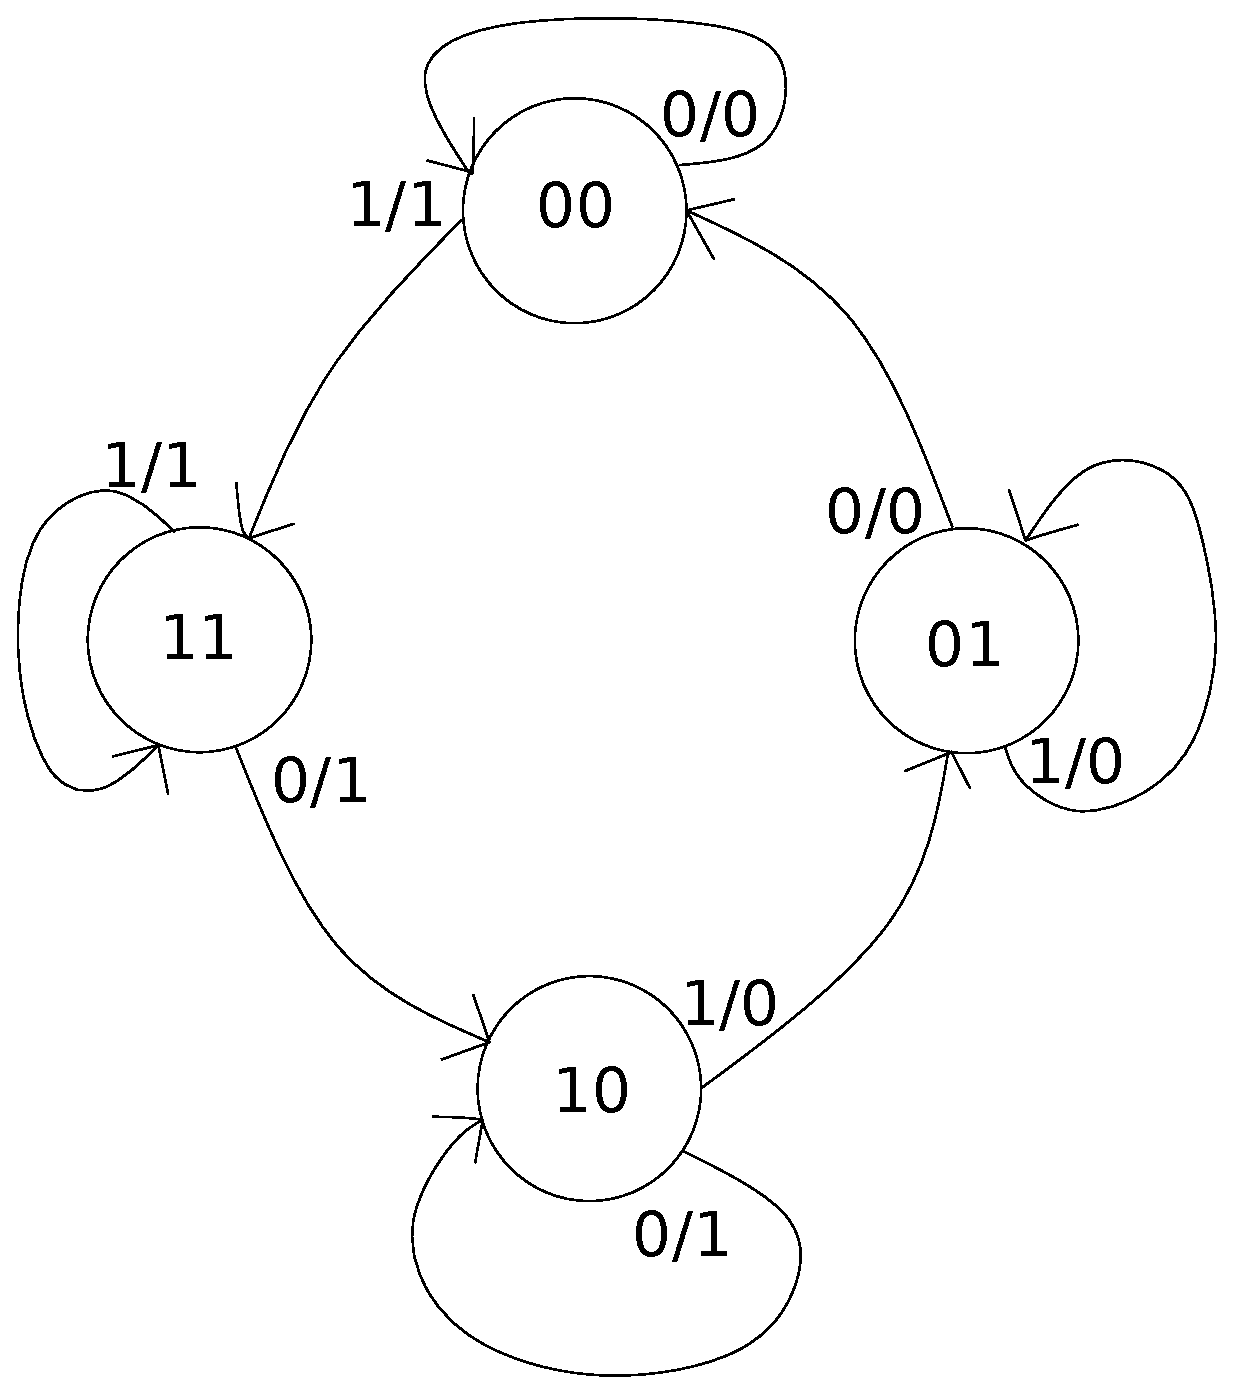
\includegraphics[scale=.3]{ex_4_1.eps}
	\caption{Exercise 1, machine state diagram}
\end{figure}

\subsection{Question 2}

The transition function $f_t$ takes in the current machine state and the input and returns the next state (so 3 bits in, 2 bits out).

\begin{table}[ht!]
	\centering
	\begin{tabular}{|c|c|c|c|}
		\hline
		BP&m1&m2&$f(BP,m1,m2)$\\\hline
		0&0&0&$(0,0)$\\\hline
		1&0&0&$(1,1)$\\\hline
		0&0&1&$(0,0)$\\\hline
		1&0&1&$(0,1)$\\\hline
		0&1&0&$(1,0)$\\\hline
		1&1&0&$(0,1)$\\\hline
		0&1&1&$(1,0)$\\\hline
		1&1&1&$(1,1)$\\\hline
	\end{tabular}
	\caption{First machine : Transition function truth table}
\end{table}

For every input, compare the state of memory to the previous table, then decide what state should be attained next clock tick depending on the button input.

\subsection{Question 3}

The output function $f_s$ takes in the state of the machine, and optionally the input, and returns the output shown by the machine. In our case, we're working with a Moore machine : the output only depends on the internal state. For our machine, it follows the following rules

\begin{table}[ht!]
	\centering
	\begin{tabular}{|c|c|}
		\hline
		State $(m1,m2)$&Output $f_s(m1,m2)$\\\hline
		$(0,0)$&$0$\\\hline
		$(0,1)$&$0$\\\hline
		$(1,0)$&$1$\\\hline
		$(1,1)$&$1$\\\hline
	\end{tabular}
	\caption{First machine, output function truth table}
\end{table}

The output is always the first bit of the memory, since it encodes the state the lamp should be in.

\subsection{Question 4}

In this case I'm assuming the "state" function is another name for the "transition" function, since that's literally the function that modifies the state. I didn't find any other instance of "state function" while scanning the handout quickly so let's run with it.

The transfer function is described by its truth table in question 2, and we find, using Karnaugh simplifications, the individual components.

The new $m_1$ is obtained using the following inputs.
\begin{table}[ht!]
	\centering
	\begin{tabular}{|c|c|c|}
		\hline
		$m_1m_2$,$BP$&0&1\\\hline
		00&0&1\\\hline
		01&0&0\\\hline
		11&1&1\\\hline
		10&1&0\\\hline
	\end{tabular}
\end{table}

So $m_1$ doesn't change if $BP$ is null, and flips if $m_2$ is not equal to $m_1$ and $BP$ is not. We find
\[
	m_1(t+1)=\overline{BP}\cdot m_1 + BP\cdot\left(m_1\cdot m_2 + \overline{m_1}\cdot\overline{m_2}\right)
\]

For $m_2$, we get
\begin{table}[ht!]
	\centering
	\begin{tabular}{|c|c|c|}
		\hline
		$m_1m_2$,$BP$&0&1\\\hline
		00&0&1\\\hline
		01&0&1\\\hline
		11&0&1\\\hline
		10&0&1\\\hline
	\end{tabular}
\end{table}

And $m_2$ is always $BP$ (since it reflects the state of the button).

So the final function is
\[
	f_t(BP,m_1,m_2)=\begin{pmatrix}\overline{BP}\cdot m_1+BP\cdot\left(m_1\cdot m_2+\overline{m_1}\cdot\overline{m_2}\right)\\BP\end{pmatrix}
\]

\subsection{Question 5}

The output function is a single bit, and from the way we have defined it, it's easily written as
\[
	f_s(m_1,m_2)=m_1
\]

\subsection{Question 6}

Finally, the following circuit should do the trick in creating this circuit. It's also in a CIRC file.

\begin{figure}[ht!]
	\centering
	\includegraphics[scale=.7]{machine_4_1.png}
	\caption{Machine for exercise 1}
\end{figure}

\section{Exercise 2}

Concevoir un système séquentiel synchrone permettant de commander l'ouverture d'une porte lorsqu'une  séquence 00, 01, 00, 10 se produit sur ses deux entrées $e1$ et $e2$. La sortie $S$ de ce système doit prendre la valeur $1$ lorsqu'une telle séquence apparaît sur ses entrées et repasser à $0$ sur la combinaison d'entrées suivante.

\centralruler

If I've undestood the question correctly, we need a system that, once it detects the given sequence of inputs, stays on for a single tick until the next input is processed.

We notice that there are in total four states in this scenario : they indicate how many elements in the sequence have been read, and what we are now waiting for. Since we're supposed to find the sequence in the last 4 inputs, it might happen that we input the beginning of the sequence multiple times and then the correct end, which should trigger the output's rise to 1 nonetheless.
If we code this correctly, we can use two bits of memory to remember how many elements along in the sequence were counted correctly and in order, and use this state plus the last input to trigger, for one clock cycle, the output.

Let us therefore use $(d2,d1)$ as memory in the following encoding
\begin{table}
	\centering
	\begin{tabular}{|c|c|}
		\hline
		Memory state & Meaning\\\hline
		$(0,0)$ & Waiting to read 00\\\hline
		$(0,1)$ & Has read 00, waiting to read 01\\\hline
		$(1,0)$ & Has read 00,01, waiting to read 00\\\hline
		$(1,1)$ & Has read 00,01,00 waiting to read 10\\\hline
	\end{tabular}
	\caption{Machine states encoding for exercise 2}
\end{table}

The state diagram is essentially a linear sequence with fallbacks to the various states if any other input that what is currently expected appears.

We find, with the inputs represented as $(e1,e2)$ that
\begin{figure}[ht!]
	\centering
	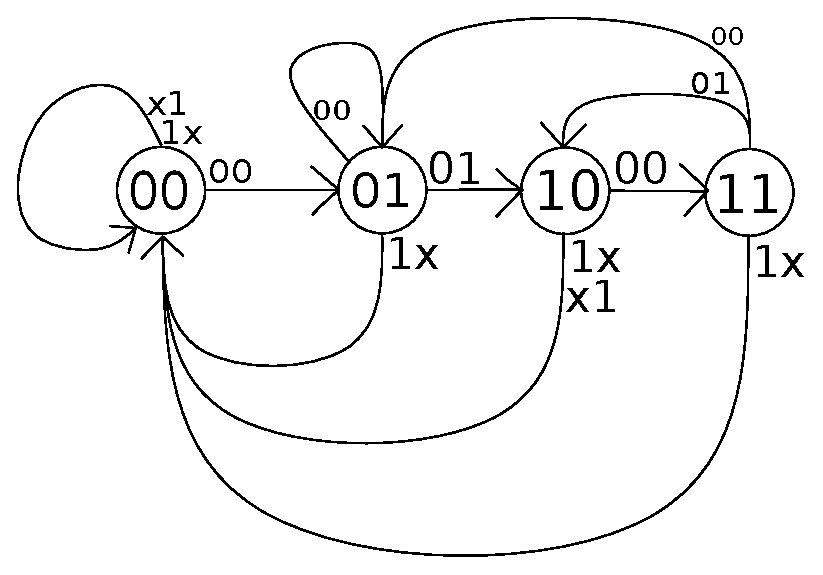
\includegraphics[scale=.4]{ex_4_2.eps}
	\caption{Machine state diagram for exercise 2}
\end{figure}

This all yields the following truth table for the transition function
\begin{table}[ht!]
	\centering
	\begin{tabular}{|c|c|c|}
		\hline
		$(e1,e2)$&$(d2,d1)$&$f_t(e1,e2,d2,d1)$\\\hline
		00&00&01\\\hline
		01&00&00\\\hline
		10&00&00\\\hline
		11&00&00\\\hline
		00&01&01\\\hline
		01&01&10\\\hline
		10&01&00\\\hline
		11&01&00\\\hline
		00&10&11\\\hline
		01&10&00\\\hline
		10&10&00\\\hline
		11&10&00\\\hline
		00&11&01\\\hline
		01&11&10\\\hline
		10&11&00\\\hline
		11&11&00\\\hline
	\end{tabular}
	\caption{Transfer function for the second machine}
\end{table}

The following are the Karnaugh tables for all three memory variables. $d3$ is systematically considered null (otherwise the system yields zero for every memory bit for the next clock tick).

First the Karnaugh table for the lowest bit of memory, $d1$.
\begin{table}
	\centering
	\begin{tabular}{|c|c|c|c|c|}
		\hline
		$(d2,d1)$|$(e1,e2)$&00&01&11&10\\\hline
		00&1&0&0&0\\\hline
		01&1&0&0&0\\\hline
		11&1&0&0&0\\\hline
		10&1&0&0&0\\\hline
	\end{tabular}
\end{table}

So $d1(t+1)=\overline{e1}\cdot\overline{e2}$.

Second, the Karnaugh table for the highest bit of memory, $d2$.

\begin{table}
	\centering
	\begin{tabular}{|c|c|c|c|c|}
		\hline
		$(d2,d1)$|$(e1,e2)$&00&01&11&10\\\hline
		00&0&0&0&0\\\hline
		01&0&1&0&0\\\hline
		11&0&1&0&0\\\hline
		10&1&0&0&0\\\hline
	\end{tabular}
\end{table}

So $d2(t+1)=\overline{e1}\cdot\left(\overline{e2}\cdot d2\cdot\overline{d1}+d1\cdot e2\right)$

Meanwhile, the output function is such that it only outputs $1$ when $(d2,d1)=(1,1)$ (read all the sequence but 10, waiting for 10), and $(e1,e2)=(1,0)$. When that happens, it gives out 1, so
\[
	f_s(d2,d1,e1,e2)=d2\cdot d1\cdot e1\cdot \overline{e2}
\]

And we can build the circuit with those elements.
We get the machine described in \autoref{fig:machine_4_2}

\begin{figure}
	\centering
	\includegraphics[scale=.5]{machine_4_2.png}
	\caption{Machine diagram for exercise 2}
	\label{fig:machine_4_2}
\end{figure}

Notice that I used a last D flip flop to stabilize the output (it was necessary here because the output would get reset after the clock tick it was supposed to appear on)

\section{Exercise 4}

On donne le graph suivant :

FIXME: mettre le graph

\textbf{Question :} Réaliser l'unité de commande correspondante avec un compteur chargeable

\centralruler{}

Let's begin by enumerating the various signals that will allow us to control the command unit (CU). There are four states given to us in this exercise, and two variales, but four different signals (one for the variables themselves, one for the complement to the variable).

Therefore we may define the following encoding table and sequencing table, shown in \autoref{tab:code_4} and \autoref{tab:seq_4}.

\begin{table}
	\centering
	\begin{tabular}{|c|c|}
		\hline
		State&Encoding\\\hline
		A&0\\\hline
		B&1\\\hline
		C&2\\\hline
		D&3\\\hline
	\end{tabular}
	\caption{State encoding table for the CU}
	\label{tab:code_4}
\end{table}

\begin{table}
	\centering
	\begin{tabular}{|c|c|c|c|c|}
		\hline
		State&Condition&Increment?&Load?&Loaded value\\\hline
		0&$\overline{C0}$&1&0&\\\hline
		1&$C1$&1&0&\\\hline
		1&$\overline{C1}$&0&1&3\\\hline
		2&&1&0&\\\hline
		3&&0&1&0\\\hline
	\end{tabular}
	\caption{State sequence table for the CU}
	\label{tab:seq_4}
\end{table}

We begin building this module in Logisim based on the one seen in the classes. We obtain the following machine, described in \autoref{fig:machine_4}.

\begin{figure}
	\centering
	\includegraphics[scale=.7]{machine_4_4.png}
	\caption{Machine diagram for the CU}
	\label{fig:machine_4}
\end{figure}

		

\end{document}
